\documentclass[12pt,convert={false}]{standalone}
\usepackage[dvipsnames]{xcolor}
\usepackage{tikz}
\usetikzlibrary{shapes,arrows,positioning,calc,patterns,arrows.meta, bending, graphs, shadings,quotes,intersections}
\usetikzlibrary{external}
%\tikzexternalize[prefix=tikz/]
\usepackage{pgfplots}
\pgfplotsset{compat=1.16}
\usepgfplotslibrary{fillbetween}
\begin{document}
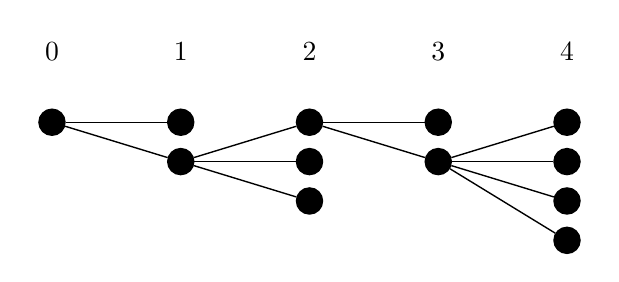
\begin{tikzpicture}[-,>=stealth', line width=0.5pt, node distance=0.5cm]
	
	\node [circle] (zero) {0};
	\node [circle, draw,circle,fill=black] (a) [below=0.4cm of zero]{};
	
	\node [circle] (one)[right=1cm of zero] {1};
	\node [circle, draw,circle,fill=black] (b) [below=0.4cm of one]{};
	\node [circle, draw,circle,fill=black] (c) [below of=b]{};
	
	\node [circle] (two)[right=1cm of one] {2};
	\node [circle, draw,circle,fill=black] (d) [below=0.4cm of two]{};
	\node [circle, draw,circle,fill=black] (e) [below of=d]{};
	\node [circle, draw,circle,fill=black] (f) [below of=e]{};
	
	\node [circle] (three)[right=1cm of two] {3};
	\node [circle, draw,circle,fill=black] (g) [below=0.4cm of three]{};
	\node [circle, draw,circle,fill=black] (h) [below of=g]{};
	
	\node [circle] (four)[right=1cm of three] {4};
	\node [circle, draw,circle,fill=black] (i) [below=0.4cm of four]{};
	\node [circle, draw,circle,fill=black] (j) [below of=i]{};
	\node [circle, draw,circle,fill=black] (k) [below of=j]{};
	\node [circle, draw,circle,fill=black] (l) [below of=k]{};
	
	\path (a) edge node [below] {} (b);
	\path (a) edge node [below] {} (c);
	
	\path (c) edge node [below] {} (d);
	\path (c) edge node [below] {} (e);
	\path (c) edge node [below] {} (f);
	
	\path (d) edge node [below] {} (g);
	\path (d) edge node [below] {} (h);
	
	\path (h) edge node [below] {} (i);
	\path (h) edge node [below] {} (j);
	\path (h) edge node [below] {} (k);
	\path (h) edge node [below] {} (l);
\end{tikzpicture}
\end{document}
